\documentclass[10pt,a4paper]{article}
\usepackage[margin=2.2cm]{geometry}
\usepackage{fontspec}
\usepackage{kotex}
\setmainfont{Apple SD Gothic Neo}
\setsansfont{Apple SD Gothic Neo}
\usepackage{amsmath,amssymb}
\usepackage{graphicx}
\usepackage{booktabs}
\usepackage{caption}
\usepackage[dvipsnames]{xcolor}
\usepackage[colorlinks=true,linkcolor=MidnightBlue,citecolor=MidnightBlue,
            urlcolor=MidnightBlue]{hyperref}
\usepackage{titlesec}
\titleformat{\section}{\large\bfseries}{\thesection}{0.6em}{}
\titleformat{\subsection}{\normalsize\bfseries}{\thesubsection}{0.5em}{}
\captionsetup{font=small,labelfont=bf}
\setlength{\parskip}{0.35em}
\setlength{\parindent}{0pt}

\usepackage{mdframed}
\newmdenv[linewidth=0.4pt,linecolor=gray!60,backgroundcolor=gray!5,
          innertopmargin=6pt,innerbottommargin=6pt,skipabove=8pt,skipbelow=8pt]{claimbox}
\newcommand{\claim}[2]{\begin{claimbox}\textbf{주장.} #1\par\smallskip
  \textcolor{gray!70}{\textbf{반증 조건.} #2}\end{claimbox}}

\title{\bfseries 태그는 양쪽으로 거짓말한다\\[2pt]
\large 표본 대신 전수를 센 이유}
\author{월드모델 실험실 · 노트 667}
\date{2026-08-06}
\begin{document}\maketitle

\section{한 줄}

라벨을 캘 수 있나를 재려고 표본 20건을 뽑았는데, 표본이 \textbf{내 계산 방법이
틀렸다}는 것을 먼저 잡아 줬다. 고쳐 세니 사전등록의 ``표본을 늘려라'' 분기였고,
표본을 늘리는 대신 \textbf{모집단 92건을 전수 열거}했다 --- 드라이브를 열기 전에,
레코드 안의 문서 목록만으로. 결과는 새 라벨 \textbf{0건}이고 채굴 경로를 닫았다.

\section{왜 이걸 했나}

노트 663 이 열값(축 하나가 판에서 물어 가는 $\rho$)이 \textbf{학습 행 수에만}
달렸음을 확정했다 --- 빈 열은 정확히 $0.0000$ 이다. 노트 665 는 팝업이 판에서
유일하게 \textbf{유보($65$)가 학습($24$)보다 큰} 도메인임을 쟀다. 노트 666 은 학습
구간(2024)에 팝업 레코드가 117건 있는데 방문객 값은 25건뿐이라고 셌다.

즉 \textbf{92건이 캘 여지}처럼 보였다. 다 캐면 학습 $24 \to 116$ 이고 열값이
크게 준다. 그런데 전례가 낮다 --- 노트 634 는 192건에서 확실한 라벨 \textbf{1건},
노트 635 는 이미지 PDF 77건에서 \textbf{4건}이다. 그래서 전수 채굴 전에
\textbf{수확률을 먼저 재기로} 사전등록했다: 고정 씨앗 20건, 문턱 20\%/10\%,
그 사이면 표본을 40으로 늘린다.

\section{표본이 나를 먼저 잡았다}

표본 20건에서 \verb|kind == '결과보고서'| 인 문서를 세니 \textbf{0/20} 이었다.
그 숫자가 너무 깨끗해서 문서 목록을 직접 열어 봤다. 그랬더니

\begin{center}
\verb|{'doc_id': '...', 'kind': '운영일지',|
\verb|'title': '(sweetspot)포켓몬고_결과보고서.pptx'}|
\end{center}

\textbf{결과보고서 파일의 태그가 `운영일지'였다.} 태그로 거르면 하나도 못 찾는다.
고쳐 세면 20건 중 \textbf{3건}이고, 그것은 사전등록 분기 ③(2$\sim$4건이면 표본을
40으로 늘린다)이다.

\claim{메타데이터 오류는 \textbf{양방향}이다. 노트 635 는 결과보고서로 태그된 파일
77건 중 \textbf{56건(73\%)이 요건정의서}임을 쟀다 --- \emph{있다고 하는데 없다}.
노트 667 은 반대다 --- 제목이 결과보고서인 실제 파일 43건의 \texttt{kind} 가 전부
\emph{운영일지}다. \emph{없다고 하는데 있다.} 그래서 태그는 \textbf{근거로도 못 쓰고
거르는 데도 못 쓴다}.}
{같은 저장소에서 \texttt{kind} 가 제목과 일치하는 비율이 높게 측정되면 이 주장은
과장이다. 다만 이번 43건은 100\% 불일치라 표본 오차로 설명되지 않는다.}

\begin{figure}[t]\centering
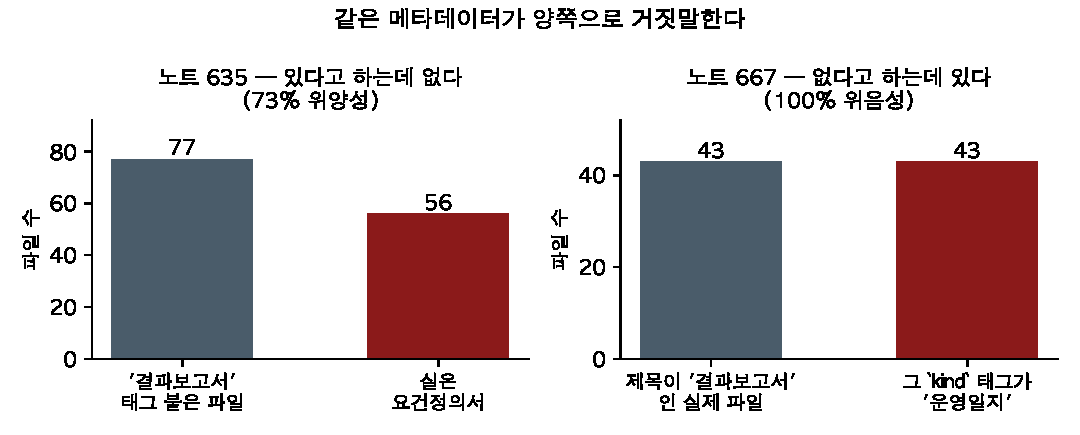
\includegraphics[width=0.98\textwidth]{figs/bothways.pdf}
\caption{같은 메타데이터가 양쪽으로 틀린다. 왼쪽(노트 635)은 위양성 73\%,
오른쪽(노트 667)은 위음성 100\%. 위양성만 겪으면 ``열어서 확인하라''로 끝나지만
위음성은 \textbf{열 후보 자체를 지운다} --- 더 조용하고 더 나쁘다.}
\end{figure}

\section{표본을 늘리는 대신 전수를 셌다}

사전등록은 ``표본을 40으로 늘린다''였다. 그런데 걸림돌이 사라졌다 --- 태그가 아니라
\textbf{제목 문자열}로 세면 그 계산은 \emph{레코드 파일 안에서} 끝난다. 드라이브를
한 번도 안 열고 92건 전수를 셀 수 있다. 40건 표본보다 강하고 비용은 더 싸다.

92건의 문서 5{,}020건을 종류로 가르면 계약서 461 · 정산 279 · 기획서 229 · 기타 106 ·
운영일지 72 다. 그 운영일지 72건 중 \textbf{29건이 \texttt{결과보고서\_내용없음.txt}}
(0바이트 플레이스홀더)이고 실제 파일은 43건, 레코드로는 \textbf{24/92 (26\%)} 다.

\begin{figure}[t]\centering
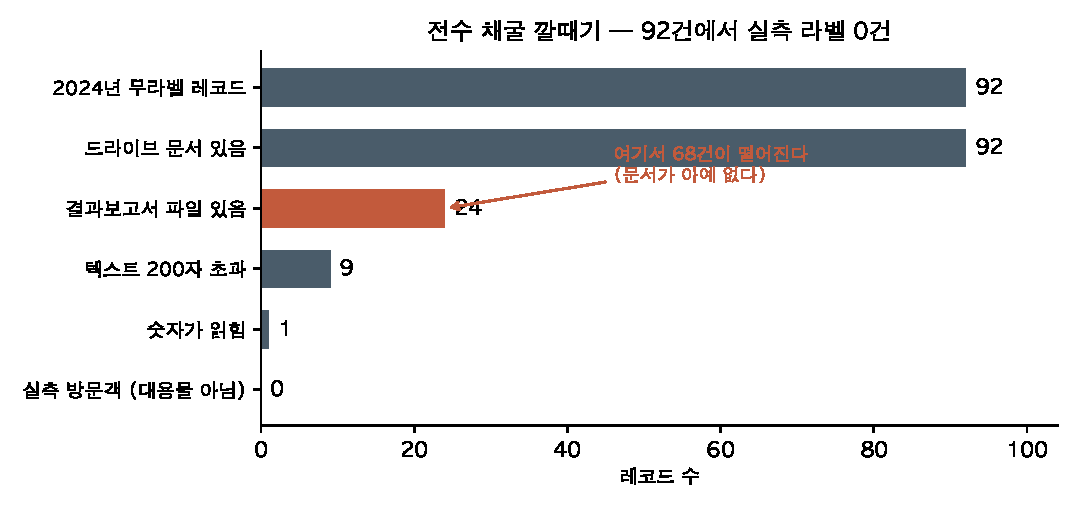
\includegraphics[width=0.86\textwidth]{figs/funnel.pdf}
\caption{24건의 43개 문서를 전부 읽었다(읽기 전용). 텍스트 200자 초과 9 ·
이미지 PDF(23$\sim$152자) 8 · jpeg 사진 14장 · 404 삭제 8 · 0바이트 txt 1 ·
비용 xlsx 1. 숫자가 읽힌 것은 한 건(\texttt{RXPU2417})이고 그것도 참가자
$746+483$ · 설문 응답자 818 로 \textbf{하한값}이다.}
\end{figure}

jpeg 14장은 연락지로 붙여 전부 봤다. \textbf{모두 현장 사진}이었다 --- 부스 조명,
크로스워크 바닥 시트, 굿즈 배치. 파일 이름이 그것을 그대로 말한다:
\verb|RTPU2446_..._결과보고서_사진대체.jpeg|.

\section{판정 --- 사전등록 분기 ②}

새 라벨은 \textbf{0건}이다. 이미 노트 634·635 가 비전으로 캔 2건(\verb|RXPU2407|
23{,}823 · \verb|RTPU2452| 18{,}600)이 이 24건 안에 있으므로 92건의 총 수확은
\textbf{2건 = 2.2\%} 다. 사전등록 문턱 10\% 미만 → \textbf{분기 ②: KOPIS 를
기다리는 것이 옳다}. 채굴로 늘 수 있는 학습 행은 $24 \to 26$ 이고 열값은 거의 안 준다.

\claim{병목은 채굴 노력이 아니라 \textbf{조직이 방문객을 안 센다}는 것이다. 노트
634·635 가 이미 그렇게 진단했고, 이번 전수가 \textbf{판의 학습 구간에 대해서도}
같은 것을 확정했다. 92건 중 \textbf{68건(74\%)은 캘 문서가 아예 없다}.}
{학습 구간에 결과보고서가 있는데 안 열어 본 레코드가 남아 있으면 이 주장은
성립하지 않는다. 24건 전수를 열었으므로 남은 것은 이미지 PDF 8건뿐이고,
노트 635 의 수확률 5.2\% 를 적용하면 기대 0.4건이라 문턱을 못 바꾼다.}

이것은 노트 666 의 \textbf{부분 정정}이다. 노트 666 은 92건을 ``안 캔 것''으로
읽었다. 정확히는 74\%가 \emph{캘 것이 없고} 26\%만 캘 수 있었고 그중 2건이 나왔다.
사전등록의 반증 조건 ③(``문서가 아예 없는 것이 15건 이상이면 정정한다'')이 발동했다.

\section{예측이 맞아서 아낀 것}

사전등록에 적은 예측은 분기 ②였고 맞았다. 그런데 값은 예측이 아니라 \textbf{순서}에
있었다. 노트 634 는 192건을 \emph{다 열고 나서} ``없다''를 알았다. 이번에는
레코드 안의 문서 목록으로 $92 \to 24$ 로 줄인 뒤 24건만 열었다 --- 드라이브 요청
43건이다.

\claim{\textbf{레코드에 문서 목록이 있으면 드라이브를 열기 전에 거를 수 있다.}
비싼 원천을 훑을 때 첫 질문은 ``무엇을 열까''가 아니라 ``무엇을 안 열어도 되나''다.}
{문서 목록이 실제 저장소와 어긋나면(삭제·이동) 이 방법이 과소 계수를 낸다.
실제로 이번에 404 가 8건 나왔다 --- 목록에는 있고 파일은 없다. 그러므로 이 방법은
\emph{상한}을 주고, 상한이 문턱 아래일 때만 결론을 낸다. 여기서는 $24 < $ 문턱이라
방향이 안전한 쪽이다.}

\section{남긴 것}

\begin{itemize}
\item 승인 대기에 \verb|RXPU2417| \textbf{하한 818} 을 올렸다. 하한값은 라벨로
      쓰면 편의가 생기므로 노트 635 의 선례대로 \textbf{사람이 정한다}. 레코드에는
      쓰지 않았다.
\item 이미지 PDF 8건은 비전으로 안 읽었다. 기대 0.4건이라 판정을 못 바꾼다.
      다만 \textbf{0 이라고 단정하지 않는다} --- 태그 오류율을 다시 잴 때 같이 넣는다.
\item 코드에 물린 것 둘: 감사의 메타 신뢰 항목에 \textbf{양방향} 오류를 적었고,
      \verb|DriveText.meta()| 를 더해 \verb|supportsAllDrives=true| 를 빼먹지
      못하게 했다. 그것이 없어 43개 문서가 전부 404 로 왔고 \emph{파일이 없는
      것처럼} 보였다 --- 이 논문의 주제가 코드에서 한 번 더 반복된 셈이다.
\end{itemize}

\end{document}
